\chapter{Visualizaci\'on de los resultados}
\label{chap:visualizacion}
\section{Herramientas}
Para visualizar la tabla de los usuarios ordenados a través de su índice $h$ y de sus centralidades
hemos recurrido al paquete Shiny de R. El código con el desarrollo de esta visualización
está en la carpeta {\bf Visualizacion/Shiny} de nuestro repositorio de GitHub.

\section{Descripción de la interfaz}
La información a mostrar al potencial cliente del proyecto es por un lado 
la lista de usuarios de Twitter susceptibles de ser candidatos a la oferta
de trabajo y por otro, de forma accesoria, el grafo que muestra la relación
entre la comunidad de usuarios identificados a lo largo del proceso de 
selección de dichos usuarios. La interfaz dispone por ello de dos pestañas, \lq\lq Listado 
de candidatos\rq\rq y \lq\lq Grafo\rq\rq:

\myfigure{
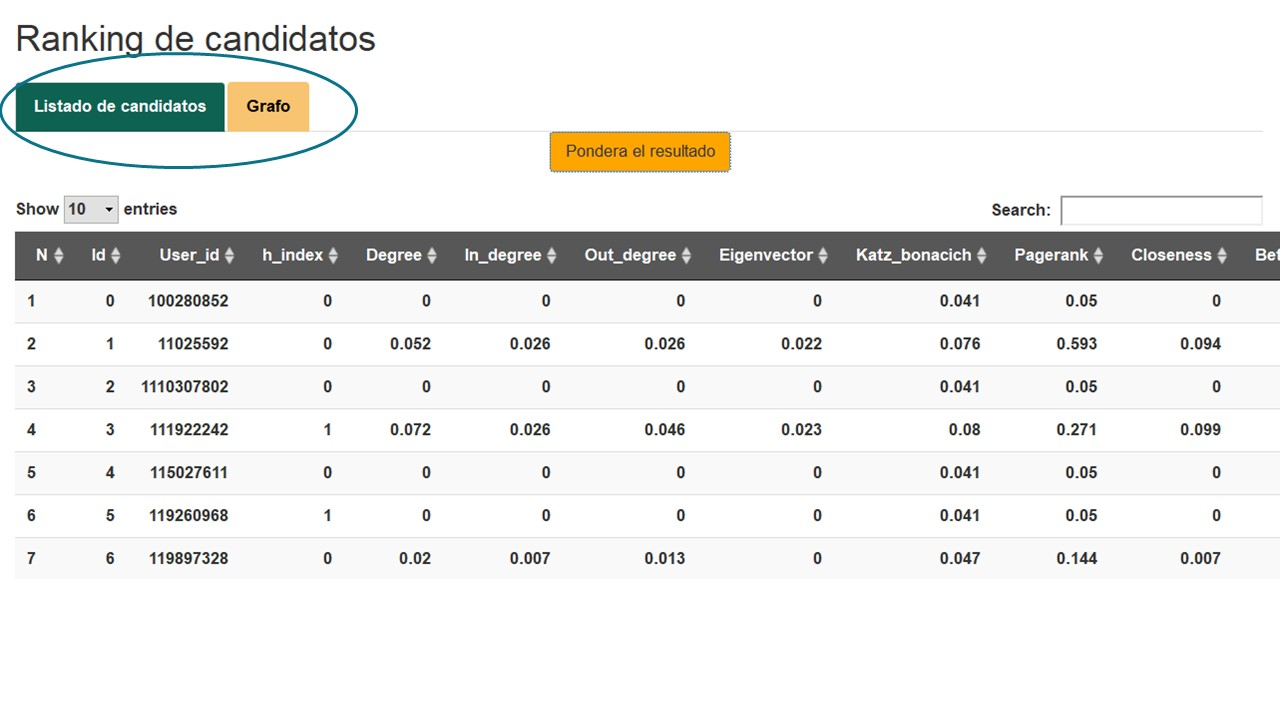
\includegraphics[width=0.8\textwidth]{Shiny_pestanas}
\figcaption{Aspecto general de la visualización, con las dos pestañas disponibles}
\label{fig:Shiny_pestanas} }

Antes de describir estas dos pestañas en detalle,
queremos hacer hincapié en que la información relativa a los usuarios siempre 
se da en relación a su \lq\lq user.id\rq\rq. 
En ningún caso proporcionamos nombres ni información obtenida personal directamente del análisis. 
En caso de querer contactar con ese usuario se tendría que hacer a través del propio Twitter y 
una vez obtenido el consentimiento del usuario a través de cualquier otra vía disponible 
(LinkedIn, blog, e-mail...)\footnote{Esta decisión la explicamos con detalle en la página 
\pageref{note:why_only_user_id}}. 



\subsection{La pestaña con la lista de usuarios ordenados: \lq\lq Listado de candidatos\rq\rq}
En esta pestaña aparece una tabla con diversos campos, comenzando
por el campo \lq\lq user.id\rq\rq que identifica al usuario, y al que siguen varias columnas 
con el índice $h$ y los diferentes tipos de centralidades. 
Las definiciones de las cantidades reflejadas en cada columna
se pueden obtener pasando el ratón por encima 
de los títulos de la tabla para que el cliente pueda tener a mano su significado sin necesidad 
de ir a otro sitio:

\myfigure{
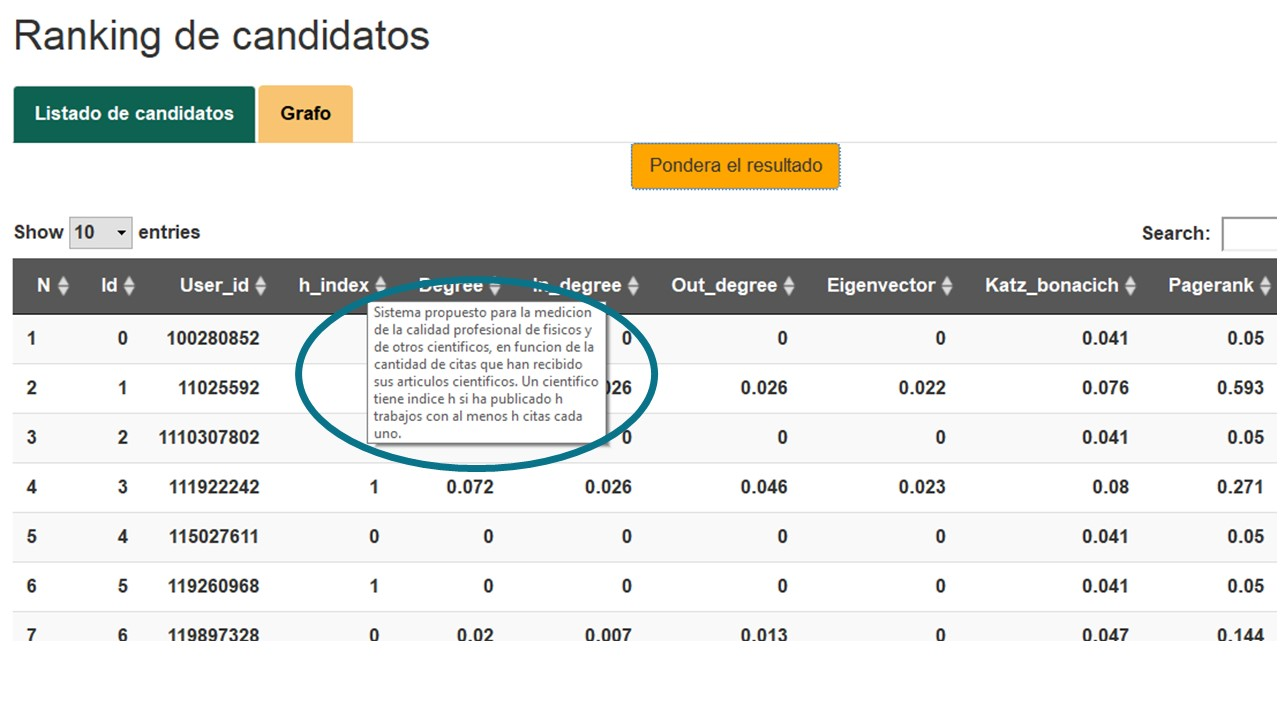
\includegraphics[width=0.8\textwidth]{Shiny_info_campos}
\figcaption{La definición de cada campo se puede ver al pasar el puntero del ratón 
por encima del título de la columna.}
\label{fig:Shiny_info_campos} }

La pestaña permite la selección del número de usuarios a mostrar por página: 
$10$, $25$, $50$ o $100$ usuarios por página:

\myfigure{
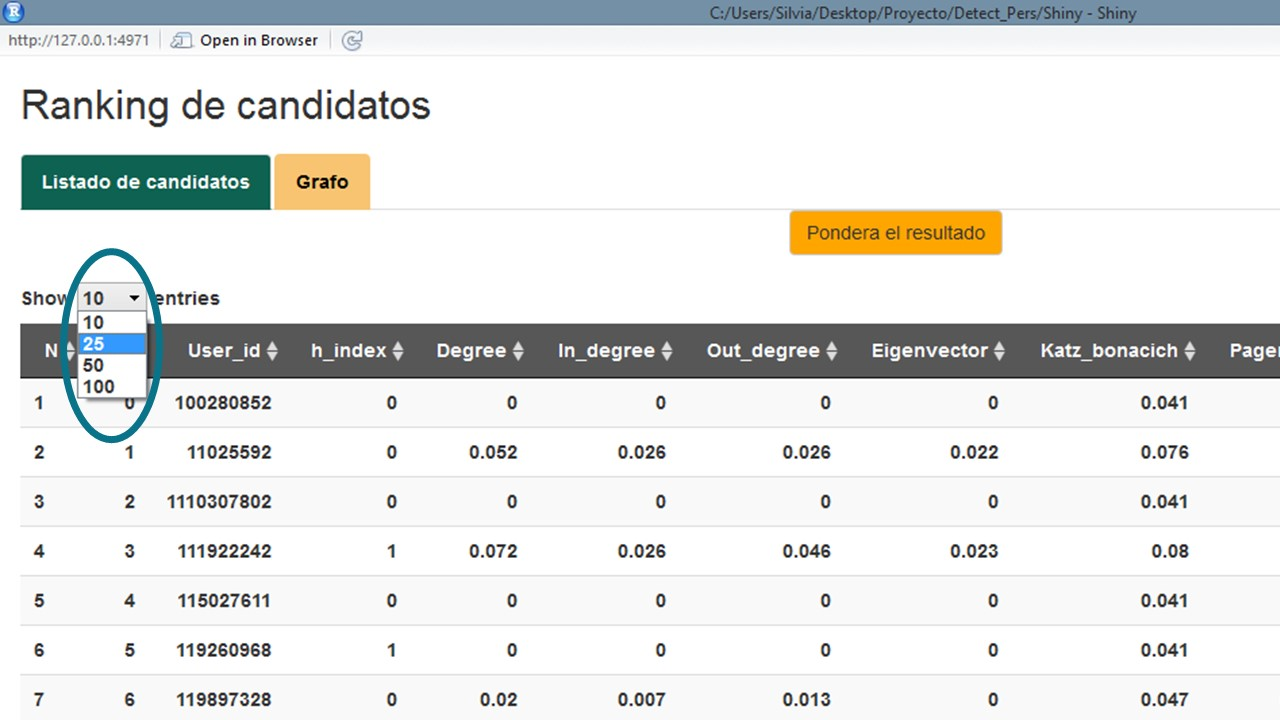
\includegraphics[width=0.8\textwidth]{Shiny_num_registros}
\figcaption{Elección del número de registros por página a mostrar.}
\label{fig:Shiny_num_registros} }

La aplicación también permite buscar por cualquier valor mostrado:

\myfigure{
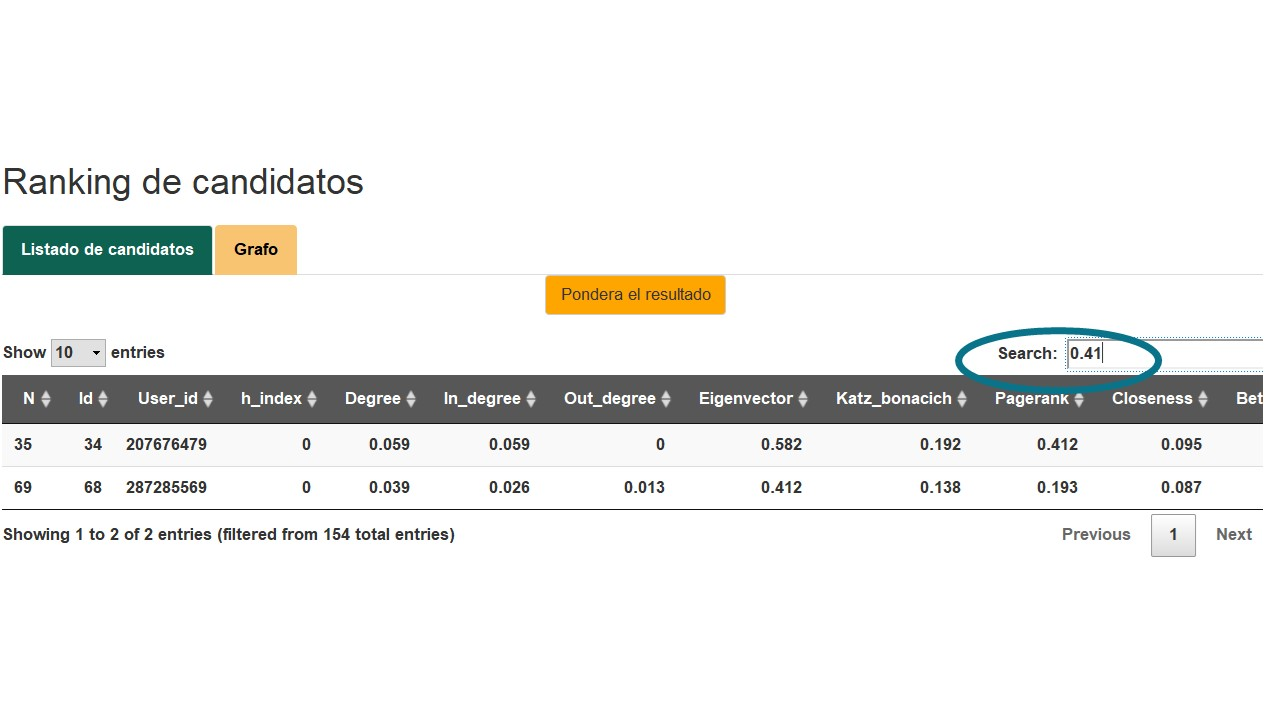
\includegraphics[width=0.8\textwidth]{Shiny_busqueda}
\figcaption{Búsqueda por valores mostrados.}
\label{fig:Shiny_busqueda} }

Para ordenar a los usuarios por los valores de alguna de las columnas, basta 
con usar las flechas que hay al lado de los nombres de las columnas (también se 
puede ordenar por varias columnas y con diferentes criterios, orden ascendente o descendente):

\myfigure{
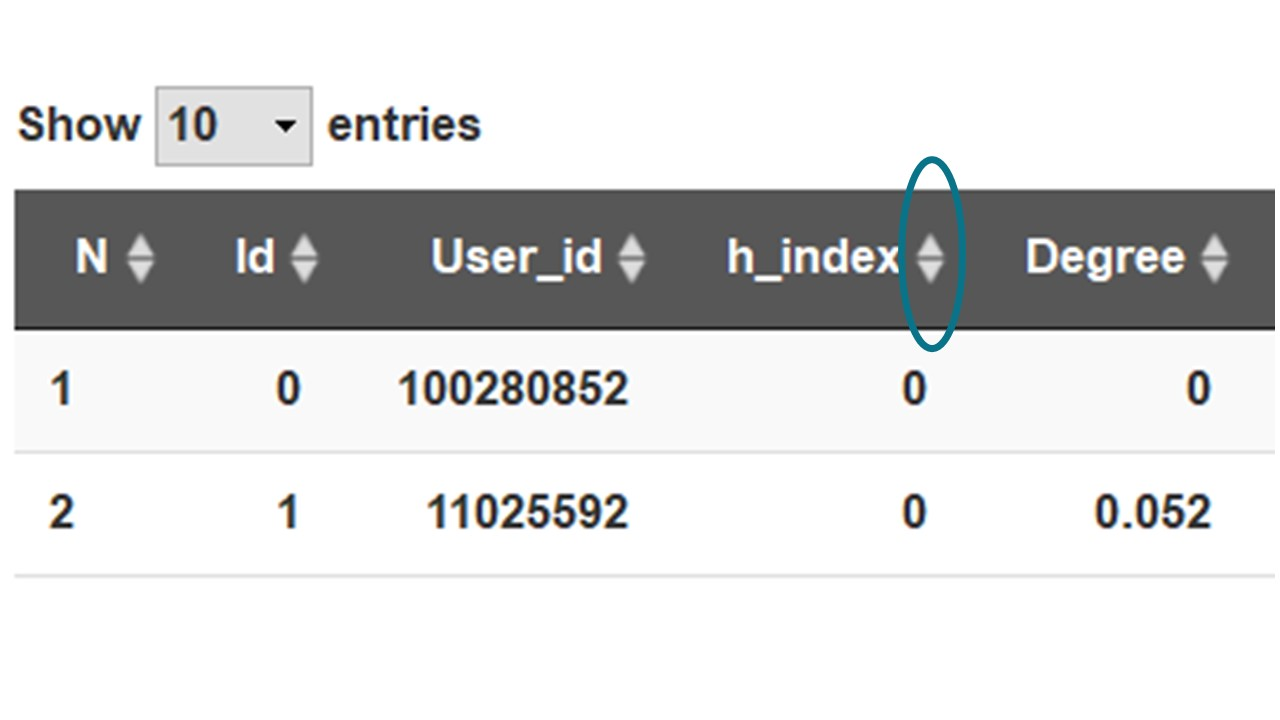
\includegraphics[width=0.5\textwidth]{Shiny_orden_1_campo}
\figcaption{Flechas para ordenar los usuarios por una única columna.}
\label{fig:Shiny_orden_1_campo} }


Además de ese orden sencillo hemos incluido una columna \lq\lq resultado\rq\rq 
donde ponderamos el resultado en función de los distintos índices que el cliente 
escoja como más relevantes para la selección adecuada del 
candidato. Para poder calcularlo adecuadamente hemos normalizado los datos ya que las escalas 
entre el índice $h$ y las centralidades era muy distintos. Hemos incluido también varios 
avisos para avisar al usuario en el caso de que los datos introducidos no sean correctos.
Para acceder a la pantalla donde poder introducir los distintos pesos, hay que hacer
click en el botón \rq\rq  Pondera el resultado\lq\lq, y aparece la siguiente pantalla:

\myfigure{
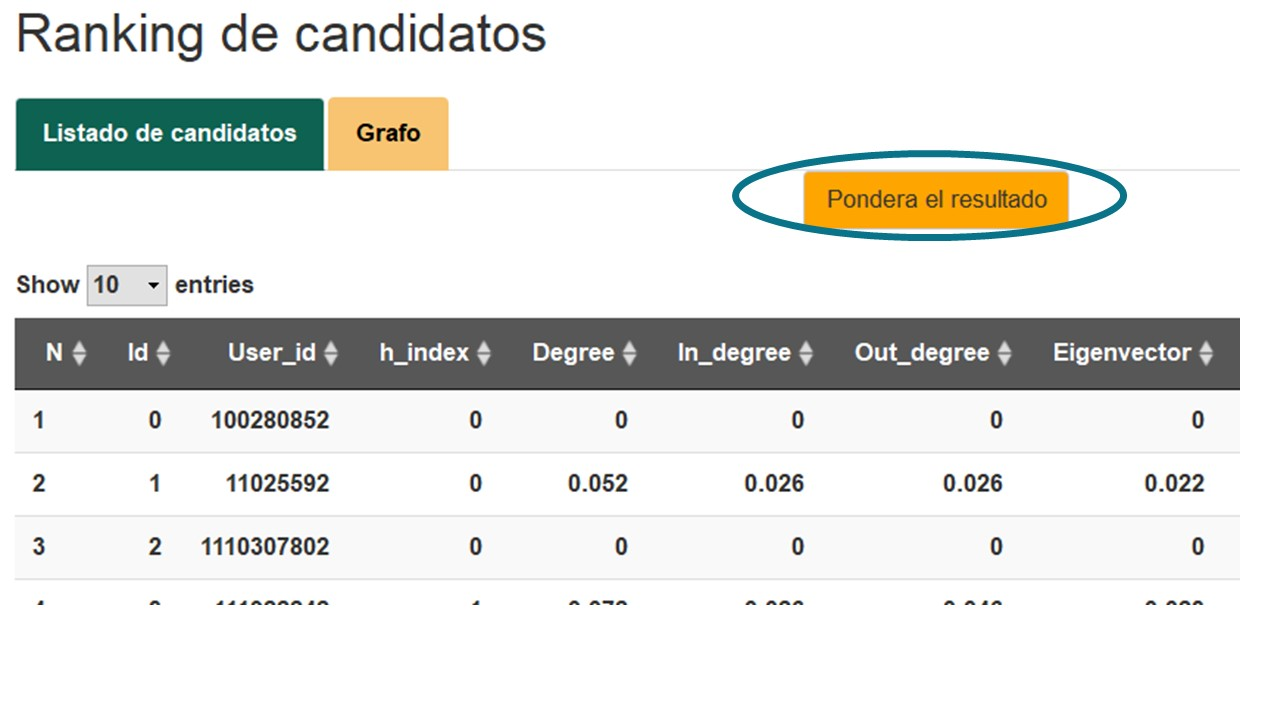
\includegraphics[width=0.5\textwidth]{Shiny_pondera_el_resultado}
\figcaption{Acceso a la pantalla para introducir los pesos.}
\label{fig:Shiny_pondera_el_resultado} }

En la ventana emergente se indica que los datos a introducir deben sumar $100$. Si por error no 
es así, vuelve a aparecer otra ventana adicional que indica que los resultados se deben revisar 
para que sumen $100$. 

\myfigure{
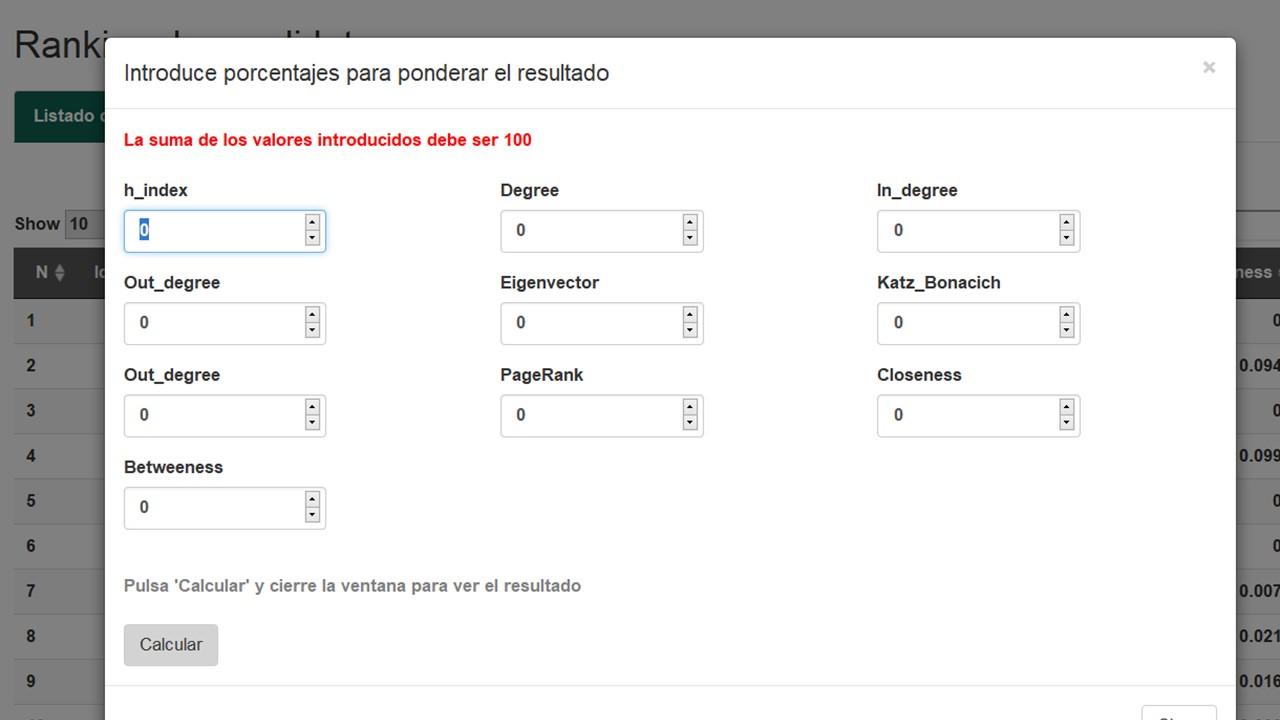
\includegraphics[width=0.5\textwidth]{Shiny_pesos}
\figcaption{Pantalla para introducir los pesos.}
\label{fig:Shiny_pesos} }

Si a pesar de ello no hacemos caso de estas advertencias en la 
página principal aparece un mensaje en rojo donde se indica claramente que la suma 
de los porcentajes no es correcta (aunque el resultado de la ponderación, sume
$100$ o no, se mostrará siempre en la columna \rq\rq  Resultado\lq\lq): 

\myfigure{
\begin{tabular}{cc}
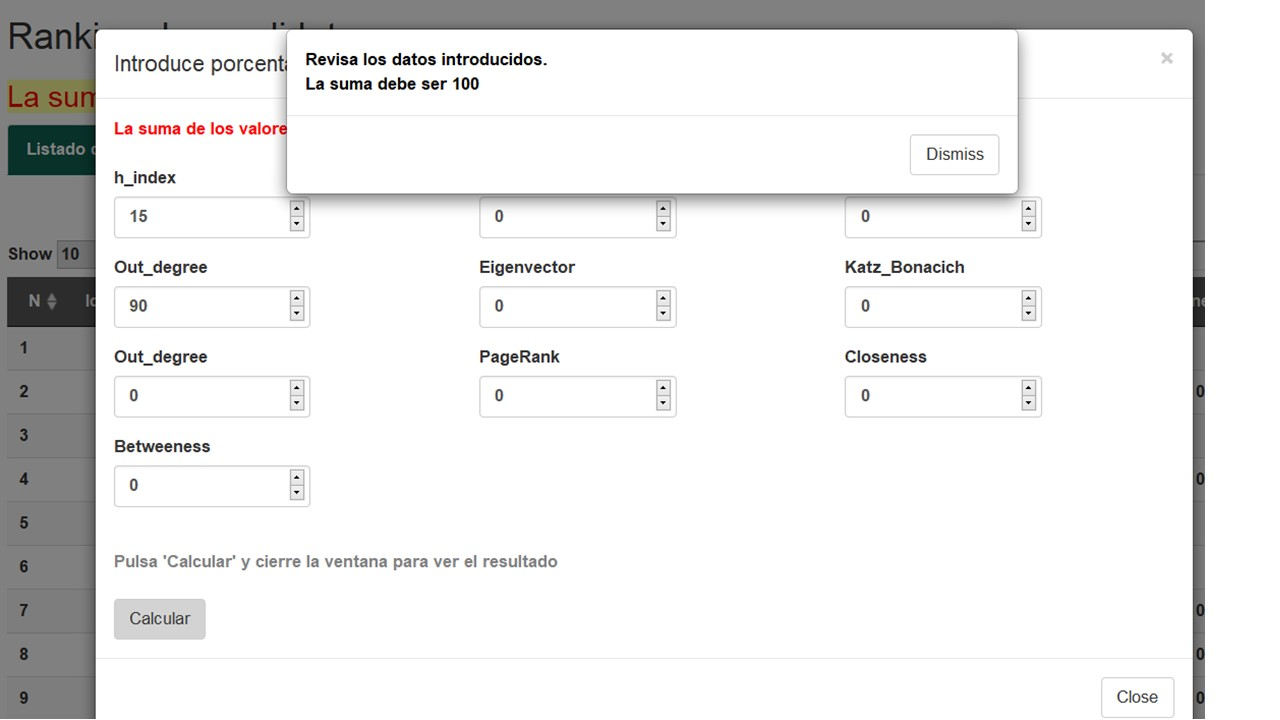
\includegraphics[width=0.45\textwidth]{Shiny_pesos_mal}
&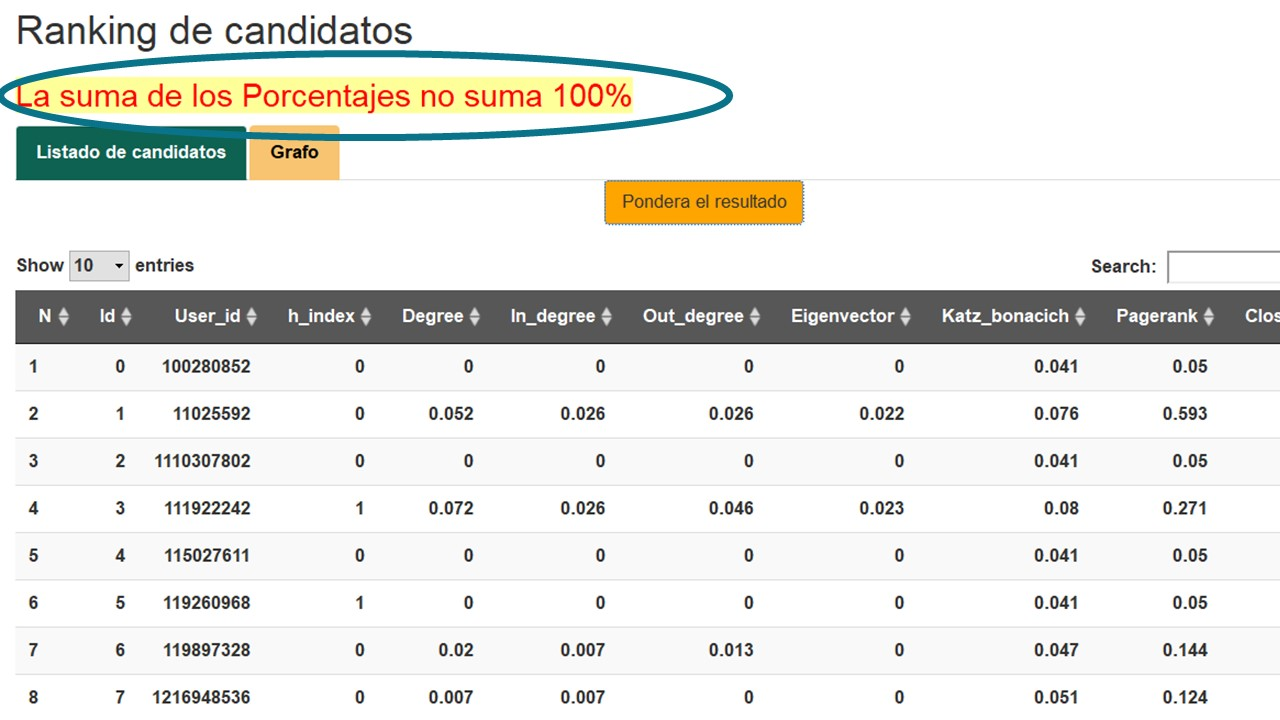
\includegraphics[width=0.45\textwidth]{Shiny_pesos_mal2}
\end{tabular}
\figcaption{Mensajes de error en el caso
de que los pesos no sean valores válidos.}
\label{fig:Shiny_pesos} }
 


\subsection{La estructura de la red: pestaña \lq\lq Grafo\rq\rq}

En la pestaña \lq\lq Grafo\rq\rq aparece una representación visual de los candidatos 
y sus relaciones:

\myfigure{
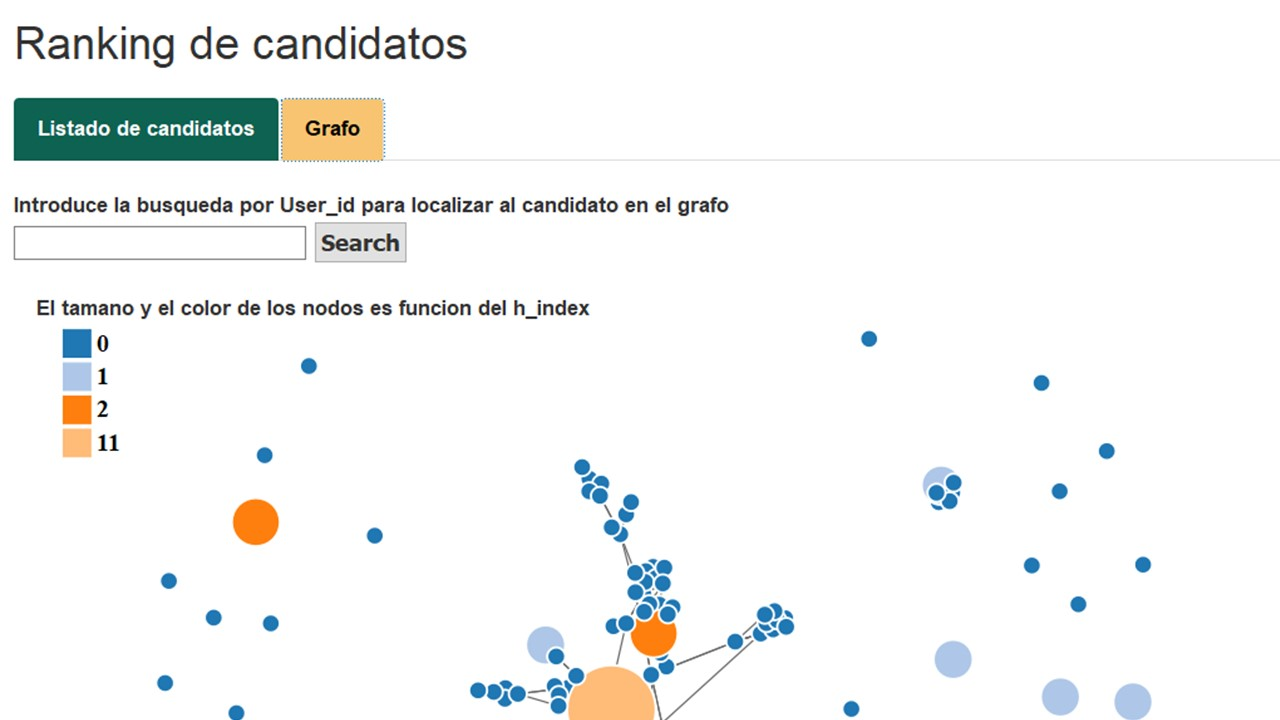
\includegraphics[width=0.8\textwidth]{Shiny_grafo1}
\figcaption{Aspecto general de la pantalla donde se muestra el grafo.}
\label{fig:Shiny_grafo1} }

Aunque el grafo que construimos con las relaciones entre los usuarios es
un grafo dirigido (tiene distinta importancia si un usuario sigue o es seguido),
la representación gráfica de ese grafo, con flechas, es bastante farragosa. 
Para mejorar la calidad gráfica, hemos elegido representar el grafo como 
un grafo no dirigido.
 
Los nodos están representados con diferentes colores y tamaños, que son función del 
índice $h$. Pasando el puntero del ratón por encima de cada nodo aparece su 
\lq\lq user.id\rq\rq:

\myfigure{
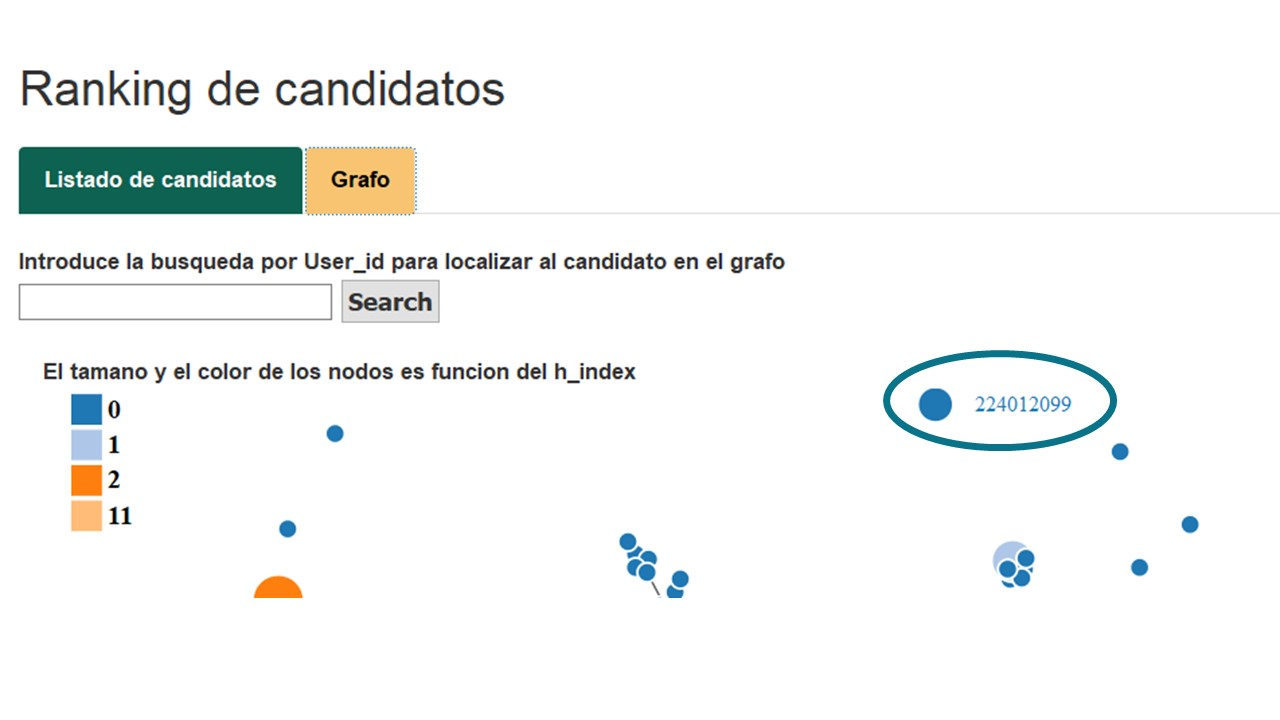
\includegraphics[width=0.8\textwidth]{Shiny_grafo_user_id_nodo}
\figcaption{\lq\lq user.id\rq\rq de un nodo por el que hemos pasado el puntero.}
\label{fig:Shiny_grafo_user_id_nodo} }

Y haciendo doble click sobre un nodo, aparece toda su información (la que 
tenemos en la tabla):

\myfigure{
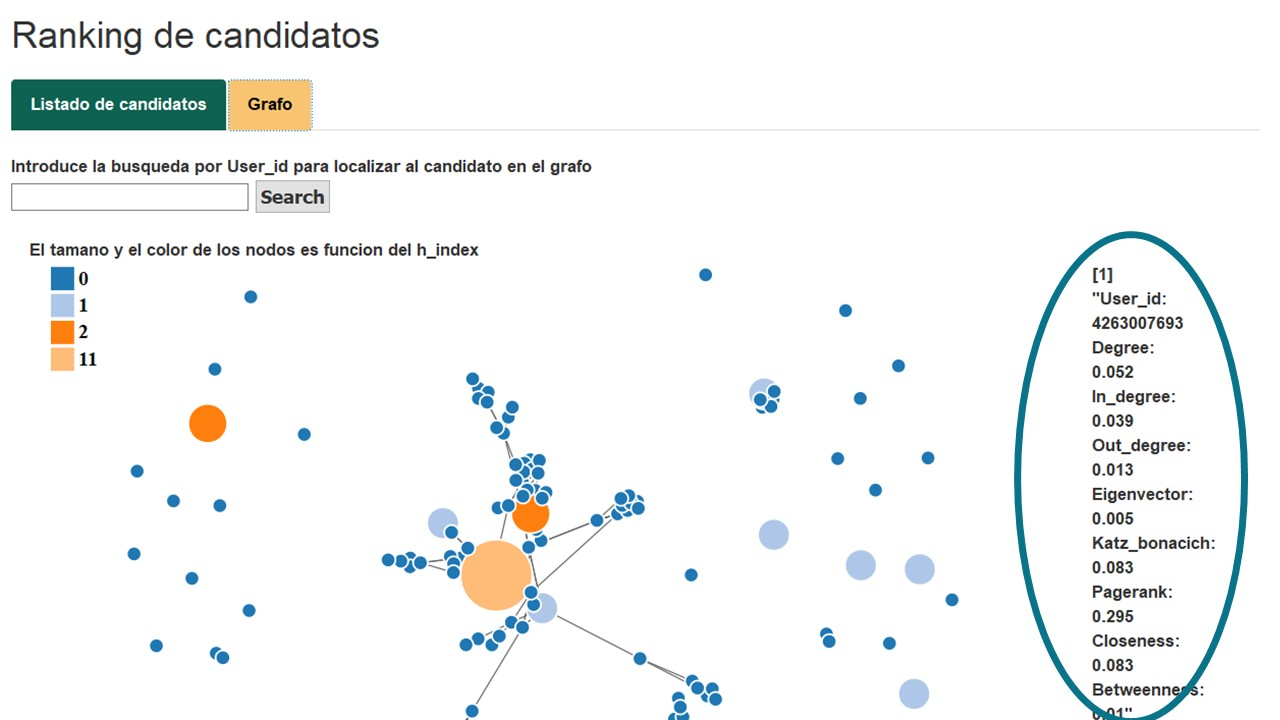
\includegraphics[width=0.8\textwidth]{Shiny_grafo_inf_nodo}
\figcaption{Información de un nodo en el que hemos hecho doble click.}
\label{fig:Shiny_grafo_inf_nodo} }

Si queremos localizar a un nodo por su \lq\lq user.id\rq\rq, podemos introducirlo en la
casilla de búsqueda y al pulsar \lq\lq Search\rq\rq, desaparecerán todos los nodos 
quedándose tan solo resaltado el nodo buscado. 
Esto durará unos segundos hasta que el grafo vuelve a aparecer normalmente:

\myfigure{
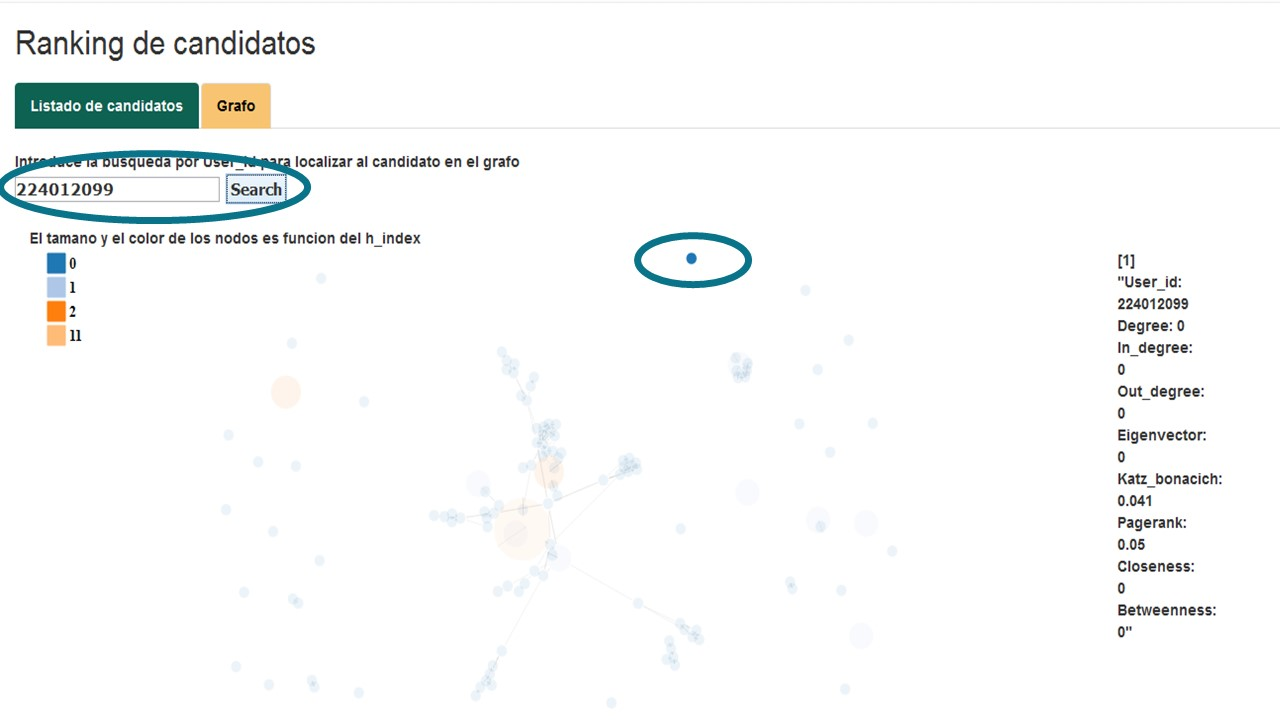
\includegraphics[width=0.8\textwidth]{Shiny_grafo_busqueda}
\figcaption{Búsqueda de un usuario en el grafo por su \lq\lq user.id\rq\rq.}
\label{fig:Shiny_grafo_busqueda} }

Del grafo cabe destacar los siguientes comentarios:
\begin{itemize}
\item Pocos nodos ($8$\%) tienen un índice $h$ igual o por encima de $1$. Teniendo en cuenta 
la definición del índice $h$ (sección \ref{subsect:indice_h}), eso significa que muchos de los 
usuarios seleccionados no tienen retuits de sus publicaciones.

\item El único usuario con un índice $h$ notable (11) tiene un in-degree de $0.039$ (no demasiado alto). 
Es decir, que este usuario no es de los que más seguidores tiene entre los usuarios destacados. Sin
embargo de sus publicaciones sobre el tema de referencia, 11 de ellas han sido retuiteadas al menos
11 veces. Además, mirando su intermediación (betweenness) tampoco es de las más altas, con lo que 
no conecta muchos de los otros usuarios entre sí. Este usuario, cuya relevancia es notable en la comunidad
general (más allá de la incluida en nuestra muestra), se captó a través de otro el cual le citaba en 
sus tuits. 


\item El usuario con mayor in-degree (mayor número de seguidores de entre los seleccionados) coincide 
con el de mayor out-degree (mayor número de amigos de entre los seleccionados). Se trata de la 
directora de una empresa del sector. 

\item El usuario con más intermediación (influencia para compartir información entre el resto de usuarios) se trata de un profesional del marketing y BI que dispone de su propio blog.


\item Varios de los usuarios con índice $h$= 1 y uno con índice $h$=2 estás \lq\lq desconectados\rq\rq de la red o casi \lq\lq desconectados\rq\rq. Esto puede ser porque el tiempo en el que duró la descarga de datos de twitter no captó al resto de sus contactos.


\item Por último mencionar que los valores tanto de \lq\lq pagerank\rq\rq como de
\lq\lq katz\_bonacich\rq\rq nunca serán igual a cero, aunque el in-degree y el out-degree del nodo 
sean cero, ya que asignan una centralidad mínima.
\end{itemize}

Para una aplicación con un número elevado de usuarios y relaciones, 
el grafo solo se mostrará para una cantidad de usuarios que aporten 
mayor relevancia en cualquiera de los índices.